\documentclass[11pt,a4paper]{article}

\usepackage[margin=2.2cm]{geometry}
\usepackage{graphicx}
\usepackage{booktabs}
\usepackage{tabularx}
\usepackage{array}
\usepackage{caption}
\usepackage{float}
\usepackage{xcolor}
\usepackage{tikz}
\usepackage[hidelinks]{hyperref}
\usetikzlibrary{arrows.meta, positioning, shapes.geometric}

\graphicspath{{../../part1/assets/brand/}{../}}

\definecolor{accent}{HTML}{0E6B67}
\definecolor{softgray}{HTML}{F4F6F6}
\definecolor{midgray}{HTML}{666666}
\definecolor{softaccent}{HTML}{E7F4F2}
\definecolor{softgold}{HTML}{FFF4D6}

\setlength{\parindent}{0pt}
\setlength{\parskip}{0.6em}
\renewcommand{\arraystretch}{1.15}
\captionsetup{labelsep=period}
\newcolumntype{L}[1]{>{\raggedright\arraybackslash}p{#1}}
\newcolumntype{Y}{>{\raggedright\arraybackslash}X}

\newcommand{\placeholder}[1]{%
    \textcolor{midgray}{\textit{[#1]}}%
}

\newcommand{\frameworknote}[2]{%
    \begin{center}
        \fcolorbox{accent}{softaccent}{%
            \begin{minipage}{0.92\textwidth}
                \textbf{#1}\\[0.35em]
                \small #2
            \end{minipage}%
        }
    \end{center}
}

\newcommand{\placeholderfigure}[3]{%
    \begin{figure}[H]
        \centering
        \fcolorbox{midgray}{softgray}{%
            \begin{minipage}[c][#2][c]{0.9\textwidth}
                \centering
                \textbf{#1}\\[0.5em]
                \small \placeholder{Insert the final artefact here.}
            \end{minipage}%
        }
        \caption{#1.}
        \label{#3}
    \end{figure}
}

\begin{document}
\pagenumbering{gobble}

\begin{titlepage}
    \centering
    \vspace*{0.2cm}
    
\includegraphics[width=4.2cm]{unsw_logo.png}

    \vspace{1.1cm}
    {\Large DESN2000 SENG\par}
    \vspace{0.3cm}
    {\Huge\bfseries Part 2 Group Report\par}
    \vspace{0.25cm}
    {\Large LaTeX Framework\par}

    \vspace{1.2cm}
    \begin{tabularx}{0.88\textwidth}{@{}L{3.2cm}Y@{}}
        Project title & \placeholder{Insert project title}\\
        Team members & \placeholder{Insert team member names and zIDs}\\
        Submission date & \placeholder{Insert submission date}\\
    \end{tabularx}

    \vfill
\end{titlepage}

\pagenumbering{roman}
\tableofcontents
\newpage
\pagenumbering{arabic}

\section{Introduction and Part 2 Scope}

\frameworknote{Section purpose}{Briefly explain that Part 2 continues from the previous user research, personas and problem definition. State that this report covers solution ideation, concept selection, backlog structure, dependencies, Sprint 1 planning, prototype traceability and Jira preparation.}

\placeholder{Insert a short introduction. Do not repeat the complete Interim Report.}

\section{Problem Statement and Research Justification}

\subsection{Problem Statement}

\frameworknote{Required content}{Insert the defined problem in a short and direct form. The statement should identify the target users, the problem they experience and the point in the journey where the problem occurs.}

\placeholder{Insert the approved problem statement.}

\subsection{Research Justification}

\frameworknote{Required content}{Briefly show how the proposed solution follows from the earlier user research, personas and problem definition. Summarise only the evidence needed to justify the design direction. Do not rewrite the complete Interim Report.}

\begin{table}[H]
    \centering
    \small
    \caption{Research-to-solution traceability template.}
    \begin{tabularx}{\textwidth}{@{}L{3.2cm}Y Y Y@{}}
        \toprule
        Research evidence & Persona or user need & Problem implication & Solution implication\\
        \midrule
        \placeholder{Evidence 1} & \placeholder{Persona or need} & \placeholder{Implication} & \placeholder{Design response}\\
        \placeholder{Evidence 2} & \placeholder{Persona or need} & \placeholder{Implication} & \placeholder{Design response}\\
        \placeholder{Evidence 3} & \placeholder{Persona or need} & \placeholder{Implication} & \placeholder{Design response}\\
        \bottomrule
    \end{tabularx}
    \label{tabresearchtraceability}
\end{table}

\section{Solution Ideation}

\subsection{Ideation Method}

\frameworknote{Required content}{Name and explain the ideation method used by the team. Show how the method started from the problem definition and produced multiple ideas. Include evidence from the actual ideation activity.}

\begin{table}[H]
    \centering
    \small
    \caption{Ideation method template.}
    \begin{tabularx}{\textwidth}{@{}L{3.1cm}Y Y Y@{}}
        \toprule
        Ideation stage & Method used & Team activity & Output\\
        \midrule
        \placeholder{Stage 1} & \placeholder{Method} & \placeholder{What the team did} & \placeholder{Produced artefact}\\
        \placeholder{Stage 2} & \placeholder{Method} & \placeholder{What the team did} & \placeholder{Produced artefact}\\
        \placeholder{Stage 3} & \placeholder{Method} & \placeholder{What the team did} & \placeholder{Produced artefact}\\
        \bottomrule
    \end{tabularx}
    \label{tabideationmethod}
\end{table}

\placeholderfigure{Ideation process and evidence}{5.2cm}{figideationevidence}

\subsection{Alternative Solution Concepts}

\frameworknote{Required content}{Present several different concepts before showing the final solution. Each concept should respond to the problem definition in a different way. Do not present only the chosen concept.}

\begin{table}[H]
    \centering
    \small
    \caption{Alternative solution concepts.}
    \begin{tabularx}{\textwidth}{@{}L{2.0cm}L{3.5cm}Y Y@{}}
        \toprule
        Concept ID & Concept name & Main idea and user value & Limitation or risk\\
        \midrule
        Concept A & \placeholder{Name} & \placeholder{Describe the concept} & \placeholder{Limitation}\\
        Concept B & \placeholder{Name} & \placeholder{Describe the concept} & \placeholder{Limitation}\\
        Concept C & \placeholder{Name} & \placeholder{Describe the concept} & \placeholder{Limitation}\\
        \bottomrule
    \end{tabularx}
    \label{tabalternativeconcepts}
\end{table}

\section{Concept Selection and Prioritisation}

\subsection{Selection Method}

\frameworknote{Required content}{Explain the systematic method used to screen and prioritise the ideas. A weighted decision matrix, MoSCoW method or another justified method may be used. Define the criteria, weights or priority rules before presenting the result.}

\placeholder{Describe the selected prioritisation method and scoring scale.}

\subsection{Decision Matrix or Prioritisation Table}

\begin{table}[H]
    \centering
    \small
    \caption{Concept selection template.}
    \begin{tabularx}{\textwidth}{@{}Y L{1.8cm}L{2.2cm}L{2.2cm}L{2.2cm}@{}}
        \toprule
        Selection criterion & Weight & Concept A & Concept B & Concept C\\
        \midrule
        \placeholder{Criterion 1} & \placeholder{Weight} & \placeholder{Score} & \placeholder{Score} & \placeholder{Score}\\
        \placeholder{Criterion 2} & \placeholder{Weight} & \placeholder{Score} & \placeholder{Score} & \placeholder{Score}\\
        \placeholder{Criterion 3} & \placeholder{Weight} & \placeholder{Score} & \placeholder{Score} & \placeholder{Score}\\
        \placeholder{Criterion 4} & \placeholder{Weight} & \placeholder{Score} & \placeholder{Score} & \placeholder{Score}\\
        \midrule
        Weighted total & 100\% & \placeholder{Total} & \placeholder{Total} & \placeholder{Total}\\
        \bottomrule
    \end{tabularx}
    \label{tabconceptselection}
\end{table}

\subsection{Selected Concept and Rationale}

\frameworknote{Required content}{Identify the selected concept and explain why it was chosen. Link the decision to the prioritisation result, user value, research evidence, feasibility and prototype scope.}

\placeholder{Insert the final concept and selection rationale.}

\section{Product Backlog Structure}

\subsection{Epic Overview}

\frameworknote{Minimum requirement}{Define at least two Epics. Every Epic must contain multiple user stories, and each story must add value to its Epic and the selected problem solution.}

\begin{table}[H]
    \centering
    \small
    \caption{Epic structure template.}
    \begin{tabularx}{\textwidth}{@{}L{1.6cm}L{4.0cm}Y L{3.0cm}@{}}
        \toprule
        Epic ID & Epic name & Epic goal and value & Linked user stories\\
        \midrule
        EP-01 & \placeholder{Epic name} & \placeholder{Epic goal} & \placeholder{US IDs}\\
        EP-02 & \placeholder{Epic name} & \placeholder{Epic goal} & \placeholder{US IDs}\\
        \placeholder{EP-03} & \placeholder{Optional Epic} & \placeholder{Epic goal} & \placeholder{US IDs}\\
        \bottomrule
    \end{tabularx}
    \label{tabepics}
\end{table}

\subsection{User Stories}

\frameworknote{Required format}{Write every story in the form: ``As a [user], I want [goal], so that [value].'' Every story must directly support the problem solution and add value to its Epic.}

\begin{table}[H]
    \centering
    \small
    \caption{User story template.}
    \begin{tabularx}{\textwidth}{@{}L{1.7cm}L{1.7cm}Y L{2.5cm}@{}}
        \toprule
        Story ID & Epic ID & User story & Priority or sprint\\
        \midrule
        US-01 & EP-01 & As a \placeholder{user}, I want \placeholder{goal}, so that \placeholder{value}. & \placeholder{Priority}\\
        US-02 & EP-01 & As a \placeholder{user}, I want \placeholder{goal}, so that \placeholder{value}. & \placeholder{Priority}\\
        US-03 & EP-02 & As a \placeholder{user}, I want \placeholder{goal}, so that \placeholder{value}. & \placeholder{Priority}\\
        US-04 & EP-02 & As a \placeholder{user}, I want \placeholder{goal}, so that \placeholder{value}. & \placeholder{Priority}\\
        \bottomrule
    \end{tabularx}
    \label{tabuserstories}
\end{table}

\section{Acceptance Criteria}

\frameworknote{Required content}{Every user story must have measurable and testable acceptance criteria. The criteria should cover the successful path and relevant validation, error, permission, privacy or edge cases. They must be suitable for later prototype or system testing.}

\subsection{Acceptance Criteria Template for Each Story}

\begin{table}[H]
    \centering
    \small
    \caption{Given-When-Then acceptance criteria template.}
    \begin{tabularx}{\textwidth}{@{}L{2.2cm}L{2.3cm}Y Y Y@{}}
        \toprule
        Acceptance ID & Scenario type & Given & When & Then\\
        \midrule
        AC-US01-01 & Success & \placeholder{Initial state} & \placeholder{User action} & \placeholder{Measurable result}\\
        AC-US01-02 & Validation or error & \placeholder{Invalid state} & \placeholder{User action} & \placeholder{Expected response}\\
        AC-US01-03 & Edge, privacy or accessibility & \placeholder{Special condition} & \placeholder{User action} & \placeholder{Expected response}\\
        \bottomrule
    \end{tabularx}
    \label{tabacceptancecriteria}
\end{table}

\frameworknote{Coverage check}{Repeat the acceptance-criteria table for every user story. Link each criterion to the relevant functional requirement, non-functional requirement and prototype screen where possible.}

\section{Functional and Non-Functional Requirements}

\subsection{Functional Requirements}

\frameworknote{Required content}{Define what the system must do. Link every requirement to one or more user stories and state how the requirement will be verified.}

\begin{table}[H]
    \centering
    \small
    \caption{Functional requirements template.}
    \begin{tabularx}{\textwidth}{@{}L{2.1cm}Y L{3.0cm}L{2.8cm}@{}}
        \toprule
        Requirement ID & Functional requirement & Related stories & Verification method\\
        \midrule
        FR-01 & The system shall \placeholder{required behaviour}. & \placeholder{US IDs} & \placeholder{Test or prototype evidence}\\
        FR-02 & The system shall \placeholder{required behaviour}. & \placeholder{US IDs} & \placeholder{Test or prototype evidence}\\
        FR-03 & The system shall \placeholder{required behaviour}. & \placeholder{US IDs} & \placeholder{Test or prototype evidence}\\
        \bottomrule
    \end{tabularx}
    \label{tabfunctionalrequirements}
\end{table}

\subsection{Non-Functional Requirements}

\frameworknote{Required content}{Include measurable requirements for privacy, security, accessibility, performance and usability. Add other categories where they are relevant to the solution.}

\begin{table}[H]
    \centering
    \small
    \caption{Non-functional requirements template.}
    \begin{tabularx}{\textwidth}{@{}L{2.1cm}L{2.5cm}Y L{2.7cm}@{}}
        \toprule
        Requirement ID & Category & Measurable requirement & Verification method\\
        \midrule
        NFR-01 & Privacy & \placeholder{Privacy target} & \placeholder{Verification method}\\
        NFR-02 & Security & \placeholder{Security target} & \placeholder{Verification method}\\
        NFR-03 & Accessibility & \placeholder{Accessibility target} & \placeholder{Verification method}\\
        NFR-04 & Performance & \placeholder{Performance target} & \placeholder{Verification method}\\
        NFR-05 & Usability & \placeholder{Usability target} & \placeholder{Verification method}\\
        \bottomrule
    \end{tabularx}
    \label{tabnonfunctionalrequirements}
\end{table}

\section{User Story Dependencies}

\frameworknote{Required content}{Identify which stories must be completed before other stories can start. Distinguish hard dependencies from optional, supporting or data relationships. The rubric checks whether these dependencies are clear.}

\subsection{Dependency Table}

\begin{table}[H]
    \centering
    \small
    \caption{User story dependency template.}
    \begin{tabularx}{\textwidth}{@{}L{2.2cm}L{3.2cm}L{2.5cm}Y@{}}
        \toprule
        Dependent story & Depends on & Dependency type & Reason\\
        \midrule
        \placeholder{US ID} & \placeholder{US ID or supporting requirement} & \placeholder{Hard, data, optional} & \placeholder{Explain the dependency}\\
        \placeholder{US ID} & \placeholder{US ID or supporting requirement} & \placeholder{Hard, data, optional} & \placeholder{Explain the dependency}\\
        \placeholder{US ID} & \placeholder{US ID or supporting requirement} & \placeholder{Hard, data, optional} & \placeholder{Explain the dependency}\\
        \bottomrule
    \end{tabularx}
    \label{tabstorydependencies}
\end{table}

\subsection{Dependency Graph}

\frameworknote{Illustrative sequence supplied in the brief}{Profile $\rightarrow$ Verification $\rightarrow$ Matching $\rightarrow$ Chat $\rightarrow$ Agreement. Replace this illustration with the validated story IDs and correct hard or optional relationships.}

\begin{figure}[H]
    \centering
    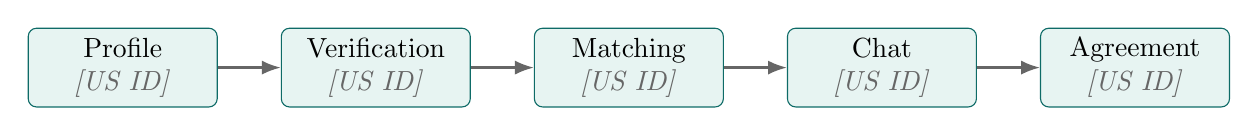
\begin{tikzpicture}[
        node distance=0.8cm,
        stage/.style={
            draw=accent,
            fill=softaccent,
            rounded corners=3pt,
            minimum width=2.4cm,
            minimum height=1.0cm,
            align=center
        },
        arrow/.style={-{Latex[length=2.4mm]}, line width=0.8pt, draw=midgray}
    ]
        \node[stage] (profile) {Profile\\\placeholder{US ID}};
        \node[stage, right=of profile] (verification) {Verification\\\placeholder{US ID}};
        \node[stage, right=of verification] (matching) {Matching\\\placeholder{US ID}};
        \node[stage, right=of matching] (chat) {Chat\\\placeholder{US ID}};
        \node[stage, right=of chat] (agreement) {Agreement\\\placeholder{US ID}};

        \draw[arrow] (profile) -- (verification);
        \draw[arrow] (verification) -- (matching);
        \draw[arrow] (matching) -- (chat);
        \draw[arrow] (chat) -- (agreement);
    \end{tikzpicture}
    \caption{First-pass user story dependency graph template.}
    \label{figstorydependencies}
\end{figure}

\section{First-Pass User Story Map}

\frameworknote{Required content}{Show the user activities, user tasks and release slices. Clearly identify which stories belong to Sprint 1 and which stories are scheduled for later sprints or the backlog.}

\begin{table}[H]
    \centering
    \scriptsize
    \caption{First-pass user story map template.}
    \resizebox{\textwidth}{!}{%
        \begin{tabular}{@{}L{2.6cm}L{2.8cm}L{2.8cm}L{2.8cm}L{2.8cm}L{2.8cm}@{}}
            \toprule
            Release slice & \placeholder{Activity 1} & \placeholder{Activity 2} & \placeholder{Activity 3} & \placeholder{Activity 4} & \placeholder{Activity 5}\\
            \midrule
            User task & \placeholder{Task} & \placeholder{Task} & \placeholder{Task} & \placeholder{Task} & \placeholder{Task}\\
            Sprint 1 & \placeholder{US IDs} & \placeholder{US IDs} & \placeholder{US IDs} & \placeholder{US IDs} & \placeholder{US IDs}\\
            Later sprint & \placeholder{US IDs} & \placeholder{US IDs} & \placeholder{US IDs} & \placeholder{US IDs} & \placeholder{US IDs}\\
            Backlog & \placeholder{US IDs} & \placeholder{US IDs} & \placeholder{US IDs} & \placeholder{US IDs} & \placeholder{US IDs}\\
            \bottomrule
        \end{tabular}%
    }
    \label{tabstorymap}
\end{table}

\subsection{Sprint 1 Scope and Rationale}

\frameworknote{Required content}{List the Sprint 1 stories and explain why they form a coherent, testable path through the selected concept.}

\placeholder{Insert the approved Sprint 1 story IDs and rationale.}

\section{Preliminary Prototype}

\subsection{Prototype Scope}

\frameworknote{Required content}{The preliminary prototype must correspond to the selected user stories. It must demonstrate the main Sprint 1 path and allow the related features to be tested.}

\placeholder{Describe the prototype scope, target users and main task flow.}

\subsection{Prototype Flow}

\placeholderfigure{Sprint 1 prototype flow}{5.2cm}{figprototypeflow}

\subsection{Prototype Screens}

\placeholderfigure{Preliminary Figma prototype screens}{8.0cm}{figprototypescreens}

\section{Prototype-to-User-Story Traceability}

\frameworknote{Required content}{Map each Figma screen to the user story and acceptance criterion that it demonstrates. Add direct frame links where available.}

\begin{table}[H]
    \centering
    \scriptsize
    \caption{Prototype-to-user-story traceability template.}
    \begin{tabularx}{\textwidth}{@{}L{1.4cm}L{2.7cm}L{2.0cm}L{2.4cm}Y L{2.5cm}@{}}
        \toprule
        Screen ID & Figma screen or frame & Story ID & Acceptance ID & Testable interaction & Figma link\\
        \midrule
        F-01 & \placeholder{Frame name} & \placeholder{US ID} & \placeholder{AC ID} & \placeholder{Interaction} & \placeholder{Frame link}\\
        F-02 & \placeholder{Frame name} & \placeholder{US ID} & \placeholder{AC ID} & \placeholder{Interaction} & \placeholder{Frame link}\\
        F-03 & \placeholder{Frame name} & \placeholder{US ID} & \placeholder{AC ID} & \placeholder{Interaction} & \placeholder{Frame link}\\
        \bottomrule
    \end{tabularx}
    \label{tabprototypetraceability}
\end{table}

\section{Jira Product Backlog}

\frameworknote{Required content}{Create the final Epics, user stories and acceptance criteria in Jira. Use the Confluence report to explain the ideation, prioritisation, mapping and prototype evidence.}

\begin{table}[H]
    \centering
    \small
    \caption{Jira backlog traceability template.}
    \begin{tabularx}{\textwidth}{@{}L{1.7cm}L{1.7cm}L{2.4cm}L{2.3cm}Y@{}}
        \toprule
        Epic ID & Story ID & Jira key or link & Sprint or status & Evidence and prototype link\\
        \midrule
        EP-01 & US-01 & \placeholder{Jira key} & \placeholder{Sprint or status} & \placeholder{Acceptance criteria and Figma link}\\
        EP-01 & US-02 & \placeholder{Jira key} & \placeholder{Sprint or status} & \placeholder{Acceptance criteria and Figma link}\\
        EP-02 & US-03 & \placeholder{Jira key} & \placeholder{Sprint or status} & \placeholder{Acceptance criteria and Figma link}\\
        \bottomrule
    \end{tabularx}
    \label{tabjirabacklog}
\end{table}

\placeholderfigure{Jira product backlog evidence}{6.2cm}{figjirabacklog}

\section{Conclusion}

\frameworknote{Section purpose}{Summarise the selected concept, the Sprint 1 scope, the preliminary prototype and the next validation step. Do not introduce new evidence in the conclusion.}

\placeholder{Insert the conclusion after the report content is complete.}

\newpage
\section{References}

\begin{itemize}
    \item \placeholder{Insert references reused from Part 1 and any new sources used in Part 2.}
\end{itemize}

\appendix

\section{Complete Acceptance Criteria}

\frameworknote{Appendix content}{Insert the complete measurable acceptance criteria for every user story.}

\section{Full User Story and Use Case Mapping}

\frameworknote{Appendix content}{Insert the final mapping between Epic IDs, user story IDs, use case IDs and requirements.}

\section{Complete Dependency Analysis}

\frameworknote{Appendix content}{Insert the final dependency table and the validated full dependency graph.}

\section{Prototype Frames and Links}

\frameworknote{Appendix content}{Insert full-size prototype frames, direct Figma links and any interaction notes needed for assessment.}

\section{Jira Evidence}

\frameworknote{Appendix content}{Insert Jira backlog exports, screenshots or links showing Epics, user stories, acceptance criteria and sprint assignment.}

\end{document}
